% Circuitos compartidos entre enunciados y solucionario
% Convención: battery1 con invert dibuja la placa larga (+) en el nodo final del trazo.

\newcommand{\circSunoQdoce}{%
\begin{circuitikz}[scale=0.9,transform shape]
\draw (0,0) to[battery1,invert,l=$\fem_1$] (0,3) to[R,l=$R_1$] (3,3)
      to[R,l_=$R_2$,*-*] (3,0) -- (0,0);
\draw (3,3) to[R,l=$R_3$] (6,3); \draw (3,0) -- (6,0) to[battery1,invert,l_=$\fem_2$] (6,3);
\node[above] at (3,3.25) {$A$}; \node[below] at (3,0) {$B$};
\end{circuitikz}}

\newcommand{\circPuente}[5]{% a-c, a-d, c-b, d-b, c-d
\begin{circuitikz}[scale=0.85,transform shape]
\coordinate (a) at (0,0); \coordinate (b) at (5,0);
\coordinate (c) at (2.5,2); \coordinate (d) at (2.5,-2);
\draw (-1,0) node[left]{$a$} to[short,o-*] (a);
\draw (b) to[short,*-o] (6,0) node[right]{$b$};
\draw (a) to[R,l=#1] (c) to[R,l=#3] (b);
\draw (a) to[R,l_=#2] (d) to[R,l_=#4] (b);
\draw (c) to[R,l=#5,*-*] (d);
\node[above] at (c) {$c$}; \node[below] at (d) {$d$};
\end{circuitikz}}

\newcommand{\circSunoQdiecinueve}{%
\begin{circuitikz}[scale=0.9,transform shape]
\draw (0,0) to[battery1,invert,l={$\fem,\ r$}] (0,3) to[R,l=$R_1$] (3.5,3) to[R,l=$R_2$,*-*] (3.5,0) -- (0,0);
\draw (3.5,3) -- (6,3) to[C,l=$C$] (6,0) -- (3.5,0);
\end{circuitikz}}

\newcommand{\circCuadrado}{%
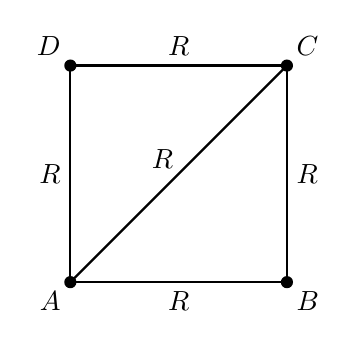
\begin{tikzpicture}[scale=1.1]
\coordinate (A) at (0,0); \coordinate (B) at (2.5,0); \coordinate (C) at (2.5,2.5); \coordinate (D) at (0,2.5);
\draw[thick] (A)--(B)--(C)--(D)--cycle; \draw[thick] (A)--(C);
\foreach \p/\n/\pos in {A/A/below left,B/B/below right,C/C/above right,D/D/above left}{\fill (\p) circle(2pt); \node[\pos] at (\p){$\n$};}
\node[below] at (1.25,0){$R$}; \node[right] at (2.5,1.25){$R$}; \node[above] at (1.25,2.5){$R$}; \node[left] at (0,1.25){$R$}; \node[above left] at (1.3,1.2){$R$};
\end{tikzpicture}}

\newcommand{\circSdosQdoce}{%
\begin{circuitikz}[scale=0.9,transform shape]
\draw (0,0) to[battery1,invert,l=$\fem_1$] (0,1.6) to[R,l=$R_1$] (0,3.4) -- (3,3.4);
\draw (3,0) to[battery1,invert,l=$\fem_2$] (3,1.6) to[R,l=$R_2$] (3,3.4);
\draw (6,1.6) to[battery1,invert,l_=$\fem_3$] (6,0);
\draw (6,1.6) to[R,l_=$R_3$] (6,3.4) -- (3,3.4);
\draw (0,0) -- (6,0);
\fill (3,3.4) circle(2pt) node[above]{$A$}; \fill (3,0) circle(2pt) node[below]{$B$};
\end{circuitikz}}

\newcommand{\circEscalera}[2]{% serie, paralelo
\begin{circuitikz}[scale=0.85,transform shape]
\draw (0,2) node[left]{$a$} to[short,o-] (0.3,2) to[R,l=#1,-*] (2.3,2) to[R,l=#1,-*] (4.6,2) to[R,l=#1,-*] (6.9,2) -- (7.6,2);
\draw (0,0) node[left]{$b$} to[short,o-] (7.6,0);
\draw (2.3,2) to[R,l=#2,-*] (2.3,0); \draw (4.6,2) to[R,l=#2,-*] (4.6,0); \draw (6.9,2) to[R,l=#2,-*] (6.9,0);
\node at (8.2,1) {$\cdots$};
\end{circuitikz}}

\newcommand{\circInterruptor}{%
\begin{circuitikz}[scale=0.85,transform shape]
\draw (-1,0) node[left]{$a$} to[short,o-*] (0,0) -- (0,1.5) to[R,l=$R$] (2.5,1.5) to[R,l=$2R$] (5,1.5) -- (5,0);
\draw (0,0) -- (0,-1.5) to[R,l_=$2R$] (2.5,-1.5) to[R,l_=$R$] (5,-1.5) -- (5,0);
\draw (5,0) to[short,*-o] (6,0) node[right]{$b$};
\draw (2.5,1.5) to[nos,l=$K$,*-*] (2.5,-1.5);
\node[above] at (2.5,1.6) {$c$}; \node[below] at (2.5,-1.6) {$d$};
\end{circuitikz}}

\newcommand{\circSdosQdiecinueve}{%
\begin{circuitikz}[scale=0.85,transform shape]
\draw (0,0) to[battery1,invert,l=$\fem$] (0,4) -- (6,4);
\draw (3,4) to[R,l=$R_1$,*-*] (3,2) to[R,l=$R_2$,-*] (3,0);
\draw (6,4) to[C,l=$C_1$] (6,2) to[C,l=$C_2$,*-] (6,0) -- (0,0);
\draw (3,2) to[nos,l=$K$] (6,2);
\node[left] at (3,2) {$c$}; \node[right] at (6.1,2) {$d$};
\end{circuitikz}}

\newcommand{\circTetraedro}{%
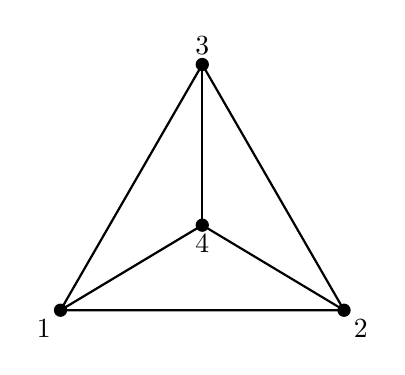
\begin{tikzpicture}[scale=1.2]
\coordinate (1) at (0,0); \coordinate (2) at (3,0); \coordinate (3) at (1.5,2.6); \coordinate (4) at (1.5,0.9);
\draw[thick] (1)--(2)--(3)--cycle; \draw[thick] (1)--(4)--(2); \draw[thick] (3)--(4);
\foreach \p/\pos in {1/below left,2/below right,3/above,4/below}{\fill (\p) circle(2pt); \node[\pos] at (\p){$\p$};}
\end{tikzpicture}}

\newcommand{\circSdosK}{%
\begin{circuitikz}[scale=0.85,transform shape]
\draw (0,0) node[below]{$G$} to[battery1,invert,l=$\fem_1$,*-] (0,2.5) to[R,l=$R_1$] (0,5) node[above]{$A$};
\draw (0,5) to[R,l=$R_2$,*-*] (8,5) node[above]{$B$};
\draw (0,5) to[R,l_=$R_3$] (4,3.2) node[below left]{$C$};
\draw (4,3.2) to[R,l_=$R_4$,*-] (8,5);
\draw (8,5) to[R,l=$R_5$] (8,0) -- (0,0);
\draw (4,0) to[battery1,invert,l=$\fem_2$,*-] (4,1.6) to[R,l=$R_6$] (4,3.2);
\end{circuitikz}}

\newcommand{\circRueda}{%
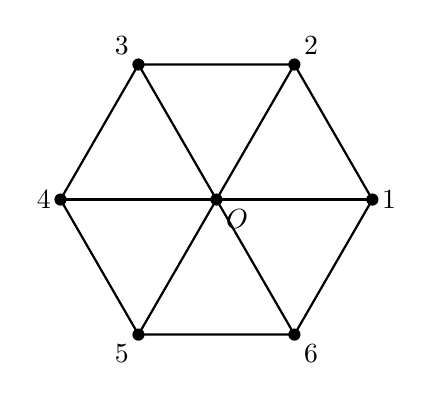
\begin{tikzpicture}[scale=1.1]
\foreach \i in {0,...,5}{\coordinate (v\i) at ({60*\i}:1.8);}
\coordinate (O) at (0,0);
\draw[thick] (v0)--(v1)--(v2)--(v3)--(v4)--(v5)--cycle;
\foreach \i in {0,...,5}{\draw[thick] (O)--(v\i); \fill (v\i) circle(2pt);}
\fill (O) circle(2pt); \node[below right] at (O){$O$};
\node[right] at (v0){$1$}; \node[above right] at (v1){$2$}; \node[above left] at (v2){$3$}; \node[left] at (v3){$4$}; \node[below left] at (v4){$5$}; \node[below right] at (v5){$6$};
\end{tikzpicture}}

\newcommand{\circInterruptoresDos}{%
\begin{circuitikz}[scale=0.85,transform shape]
\draw (-1,0) node[left]{$a$} to[short,o-*] (0,0) -- (0,1.8) to[R,l=$R$] (2.2,1.8) to[R,l=$R$] (4.4,1.8) to[R,l=$R$] (6.6,1.8) -- (6.6,0);
\draw (0,0) -- (0,-1.8) to[R,l_=$R$] (2.2,-1.8) to[R,l_=$R$] (4.4,-1.8) to[R,l_=$R$] (6.6,-1.8) -- (6.6,0);
\draw (6.6,0) to[short,*-o] (7.6,0) node[right]{$b$};
\fill (2.2,1.8) circle(2pt) node[above]{$c$}; \fill (4.4,1.8) circle(2pt) node[above]{$d$};
\fill (2.2,-1.8) circle(2pt) node[below]{$e$}; \fill (4.4,-1.8) circle(2pt) node[below]{$f$};
\draw (2.2,1.8) to[nos,l_=$K_1$] (2.2,0.3) -- (4.4,-1.8);
\draw (4.4,1.8) to[nos,l=$K_2$] (4.4,0.3) -- (2.2,-1.8);
\end{circuitikz}}

\newcommand{\circSdosCap}{%
\begin{circuitikz}[scale=0.9,transform shape]
\draw (0,0) to[battery1,invert,l=$\fem_1$] (0,1.6) to[R,l=$R_1$] (0,3.4) -- (6,3.4);
\draw (3,0) to[battery1,invert,l=$\fem_3$] (3,1.6) to[C,l=$C$] (3,3.4);
\draw (6,0) to[battery1,invert,l_=$\fem_2$] (6,1.6) to[R,l_=$R_2$] (6,3.4);
\draw (0,0) -- (6,0);
\fill (3,3.4) circle(2pt) node[above]{$A$}; \fill (3,0) circle(2pt) node[below]{$B$};
\end{circuitikz}}
